\chapter{Introduction}

\section{Motivation}
Revealing the structure of hierarchical organized data is a complex task where many approaches already exists. It is still an active research area as data scientists are facing ever greater challenges when analyzing large hierarchical datasets. One example is the Human Disease Network \cite{zhou_human_2014} which is a hierarchical network of disorders and disease genes with approximately 3000 nodes on two different hierarchy layers. Figure \ref{fig:Human_Disease_Network} shows us the representation of the data in a common two-dimensional layout. In this representation, the classes of disorders are coded by color. 
Another dataset with a similar structure can be seen in Figure \ref{fig:original2DdiseaseNet}, here the clusters of different diseases are grouped by boxes.\\ 
Depiction of hierarchical network structure in 2D faces us with many challenges. The biggest one is visual clutter also called hairball effect which reduces the legibility of the network information, therefore it is difficult to determine node-node relationships and hierarchic-associations as well as hierarchic relationships which are crucial in analyzing hierarchical network data. In Figure \ref{fig:Human_Disease_Network} we can see this effect on the green nodes. The graph in Figure \ref{fig:original2DdiseaseNet} solves this problem by hiding links between child nodes from different boxes which is also not optimal.

\begin{figure}[h]
    \centering
    \begin{subfigure}[b]{0.4\columnwidth}
        \centering
        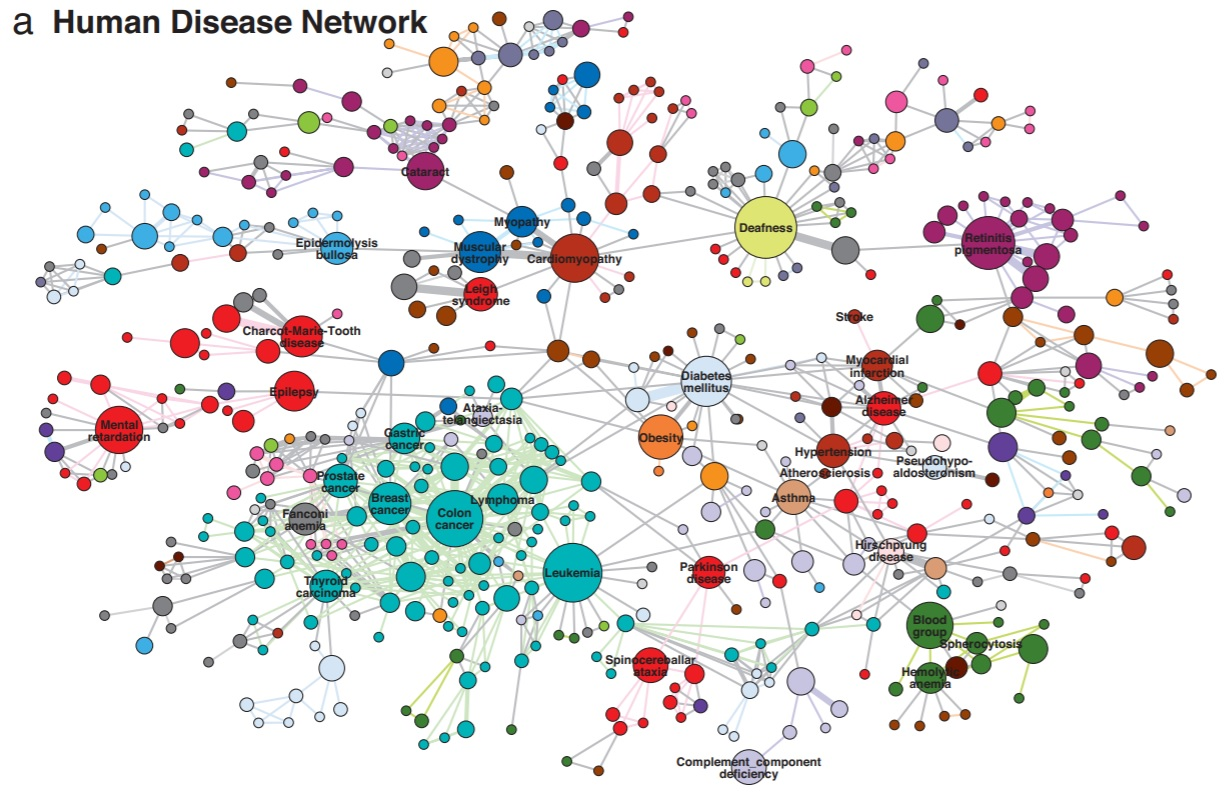
\includegraphics[width=\textwidth, trim={0 0 9cm 0},clip]{graphics/Human_Disease_Network.jpg}
        \subcaption{Human Disease Network \cite{zhou_human_2014}}
        \label{fig:Human_Disease_Network}
    \end{subfigure}
    \begin{subfigure}[b]{0.5\columnwidth}
      \centering
      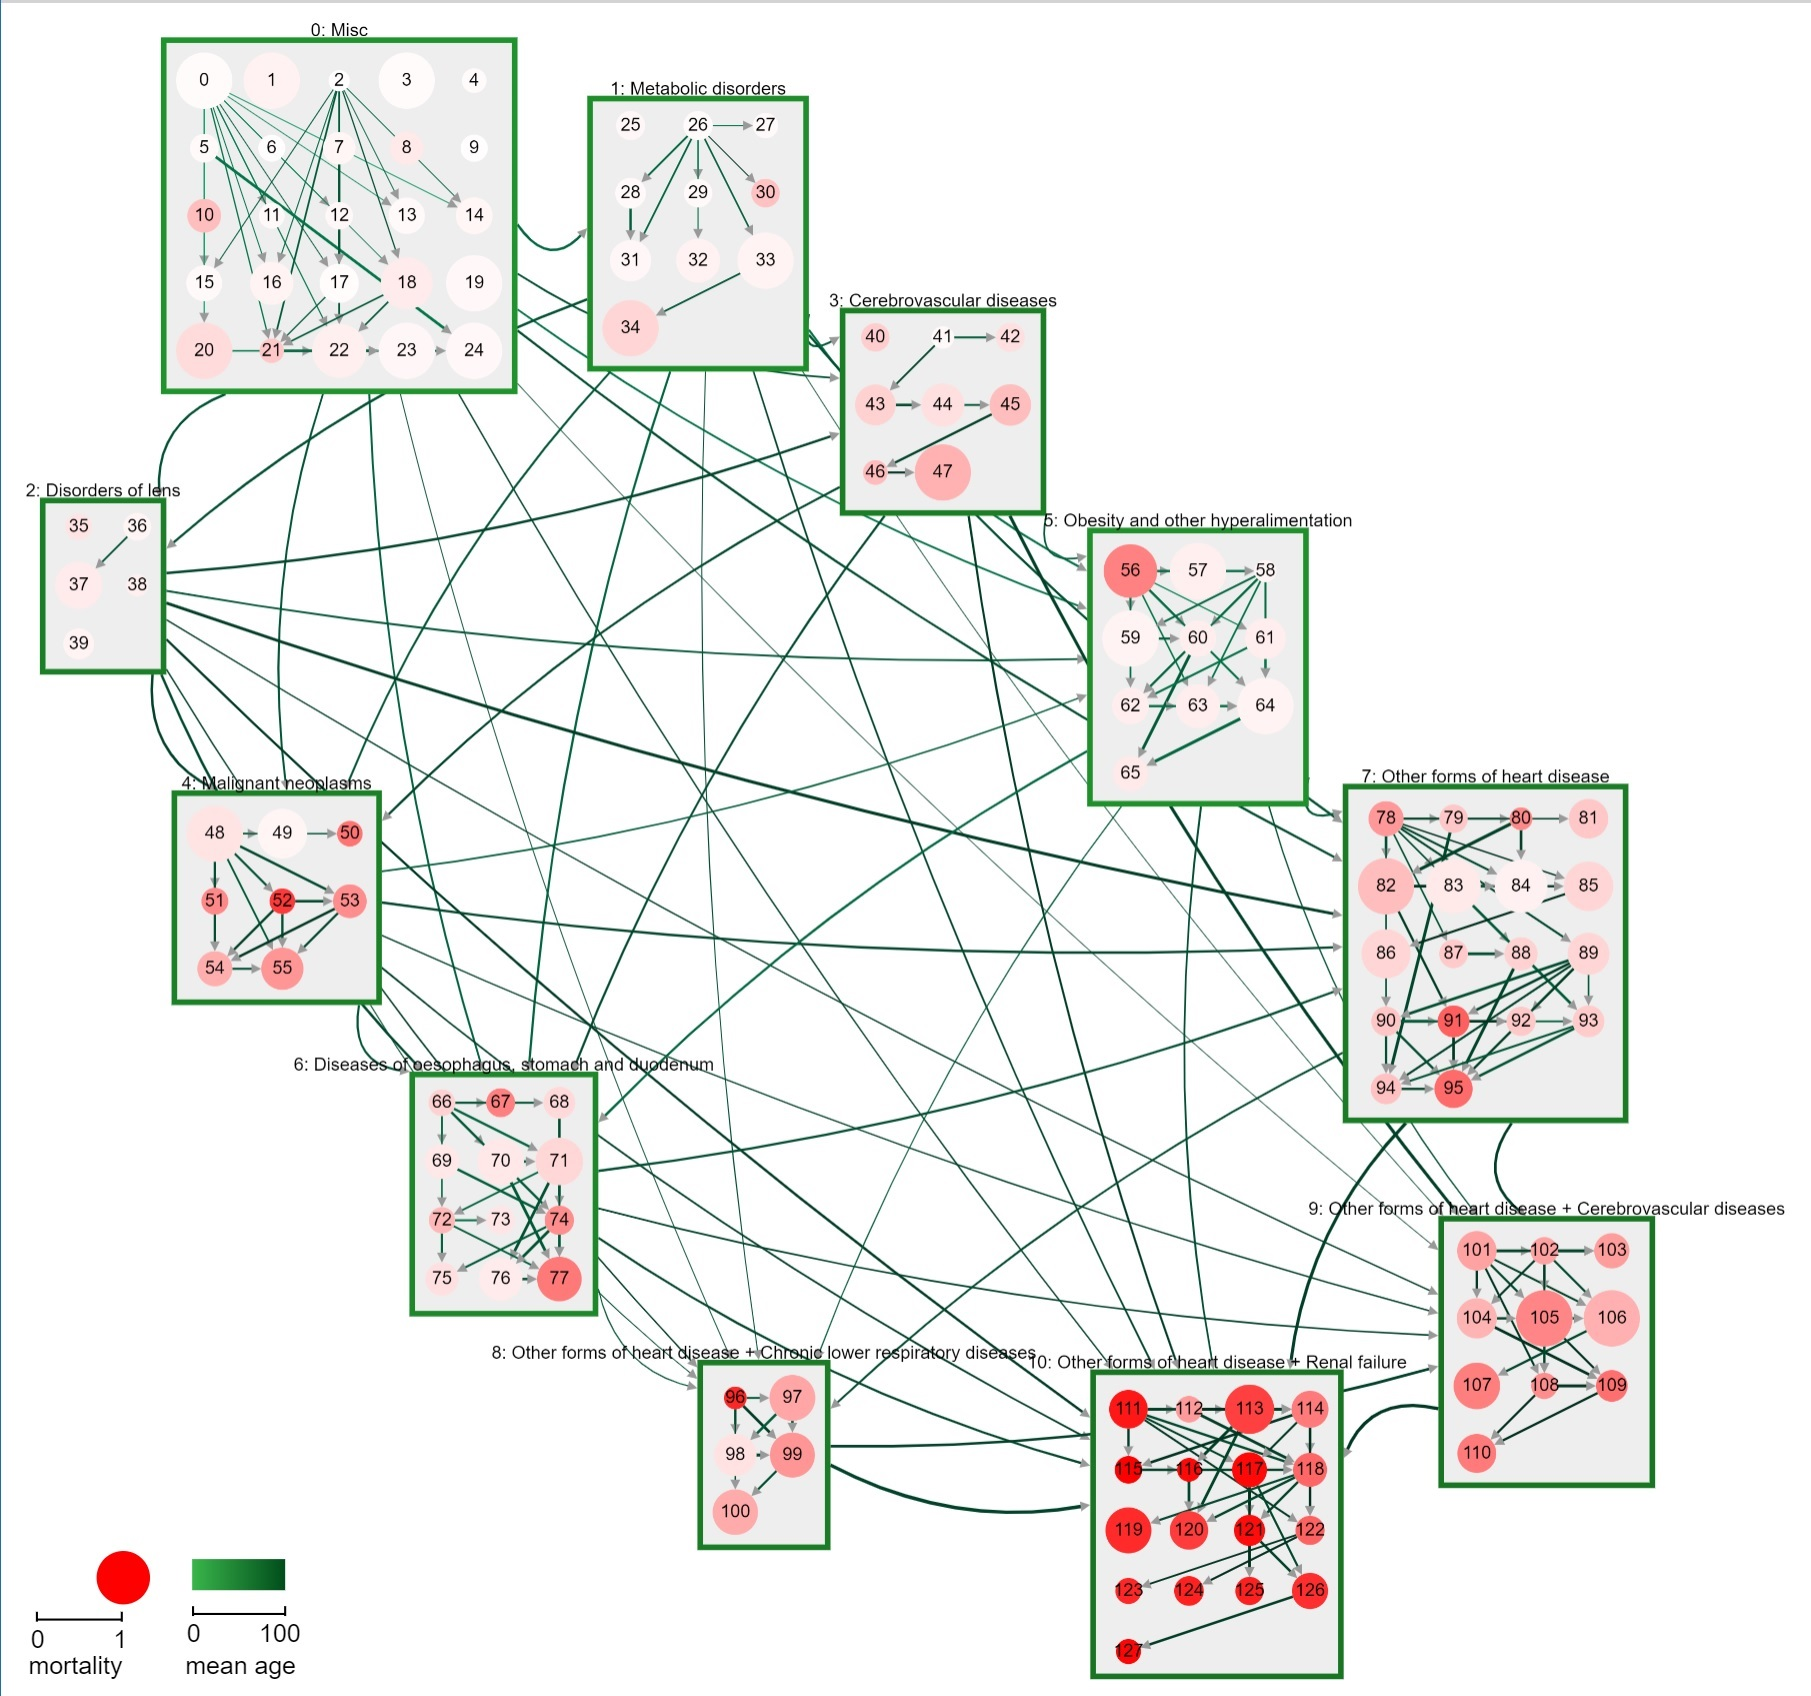
\includegraphics[width=\textwidth]{graphics/original2DdiseaseNet.jpg}
      \subcaption{a comorbidity network of diagnoses related to diabetes melitus}
      \label{fig:original2DdiseaseNet}
    \end{subfigure}
    \caption[visualizations of hierarchical network datasets.]{Example visualizations of hierarchical network datasets in two dimensions. Both consists of two hierarchical layers.} % Remove the [...] argument if the original caption should be used in the figure list.
    \label{fig:intro} 
  \end{figure}

3D information visualization allows us to expand the user experience of traditional 2D graphs. As Brath describes in his paper \cite{brath_3d_2014} there are many advantages and opportunities when using three-dimensional visualizations.
By using an additional axis the visualization has more space to distribute all the data and reduce clutter in the first place before applying specialized layouts. The mental model of the data gets improved which leads to a better cluster detection, conformation and general overview of the data. 
Some visualization also use the additional axis to encode an extra attribute by its position, this can be seen in the “3D space time cube” \cite{brath_3d_2014} here the temporal information is encoded on the Z axis another common usage is a 3D scatter plot.
In three-dimensional layouts, the perspective of the visualization has to be reconsidered. Usually the user looks from the outside with a bird's eye view at the visualization. In 3D however the viewer can be placed right inside our graph, this enables us to utilize new navigation and interaction possibilities.

Still, all these opportunities also involve new challenges: navigation inside a hierarchically structured 3D scene, occlusion of elements in an 3D perspective view, selection of objects for displaying details and the lack of a reference point in an abstract three-dimensional space. Brath \cite{brath_3d_2014} already stated that immersive interfaces could help to overcome these issues.\label{chap:advantages_VR}
We believe that the recent developments in virtual reality hardware and frameworks offer great potential to address these challenges. 
We can see the benefits of VR based visualizations in various publications. Bowman and McMahan \cite{bowman_virtual_2007} examined the impact of VR techniques, like stereoscopic images, interaction with the virtual world and head movement, can have on users. 
Recently Kraus et al. \cite{kraus_impact_2020} did a study on the effect of immersion for detecting clusters in a scatter plot. Their results show that VR based visualization systems have real world advantages in terms of time needed to get an overview of the data compared to traditional 2D- and 3D information visualization. 
 
\section{Aim of the Work}

Our goal is to implement a visualization for hierarchical network data that allows users take the benefits of 3D information visualization and opportunities of virtual reality technology to dive right into the data. We believe the combination of both concepts complement each other well because VR based technology can be used to solve the subsequent challenges from 3D information visualization and therefore enable data scientists to optimize their data analysis tasks. 
Our aim was to design a customized graph layout that calculates the position and size of each node by the hierarchical structure: child nodes are nested within their parent node. 
In addition, visual clutter by overlapping of nodes and links should be prevented. 
Furthermore, the exploration of the resulting graph should be possible with room scale virtual reality devices like the HTC Vive, requiring optimized navigation, filtering and brushing methods to enhance the graph exploration user experience.

\section{Methodology}
In order to achieve the proclaimed goal we firstly did research on already working solutions. We summarized important techniques many approaches share and categorized them into different visualization types in Section \ref{chap:rw-2d3dLayout}. 
Before improving a visualization we had to get a clear understanding of our data structure, therefore we looked into the theory behind it. Section \ref{chap:bg-graphTheory} explains the concepts of different graphs data structures, their extensions like trees but also fundamentally drawing techniques like node-link diagrams.
As we were planning a VR visualization, we also looked into VR technology from a feature perspective in Section \ref{chap:bg-vrtech}. Furthermore, we examined other related works in the field of VR visualization including navigation and interaction methods as well as VR specialized graph layouts in Section \ref{chap:rw-VRVIS}.\\
With our goal in mind we defined some requirements the visualization has to meet in order to be a success. These requirements can be found in Section \ref{chap:ps-requirements}.
To design our own visualization system we need a concept for our VR specialized layout which can be found in Section \ref{chap:ps-layout}. 
Its task is to find the node positions in order to achieve a distributed hierarchical nested graph with no node overlapping, which is primarily done by a customized force system.
Furthermore, a fitting render representation had been designed (see Section \ref{chap:ps-graphRepresentation}) as well as VR optimized interaction (see Section \ref{chap:solution-interaction}) and navigation methods (see Section \ref{chap:solution-navigation}). 
A detail description on the implementation process can be found in Chapter \ref{chap:Impl}. The resulting visualization can be seen in Figure \ref{fig:conceptSketch}.\\
For evaluation, we measured performance and technical limits of our solution in Section \ref{sec:performanceEvaluation}. In addition, we gathered informal  feedback on the usability in the form of an interview and forms in Section \ref{sec:informalFeedback}. As a side note, due to the COVID-19 pandemic during the writing we were mostly restricted to online feedback.\\
Lastly in Chapter \ref{chap:conclusion} we discuss some problems and future work.

\begin{figure}[h]
    \centering
    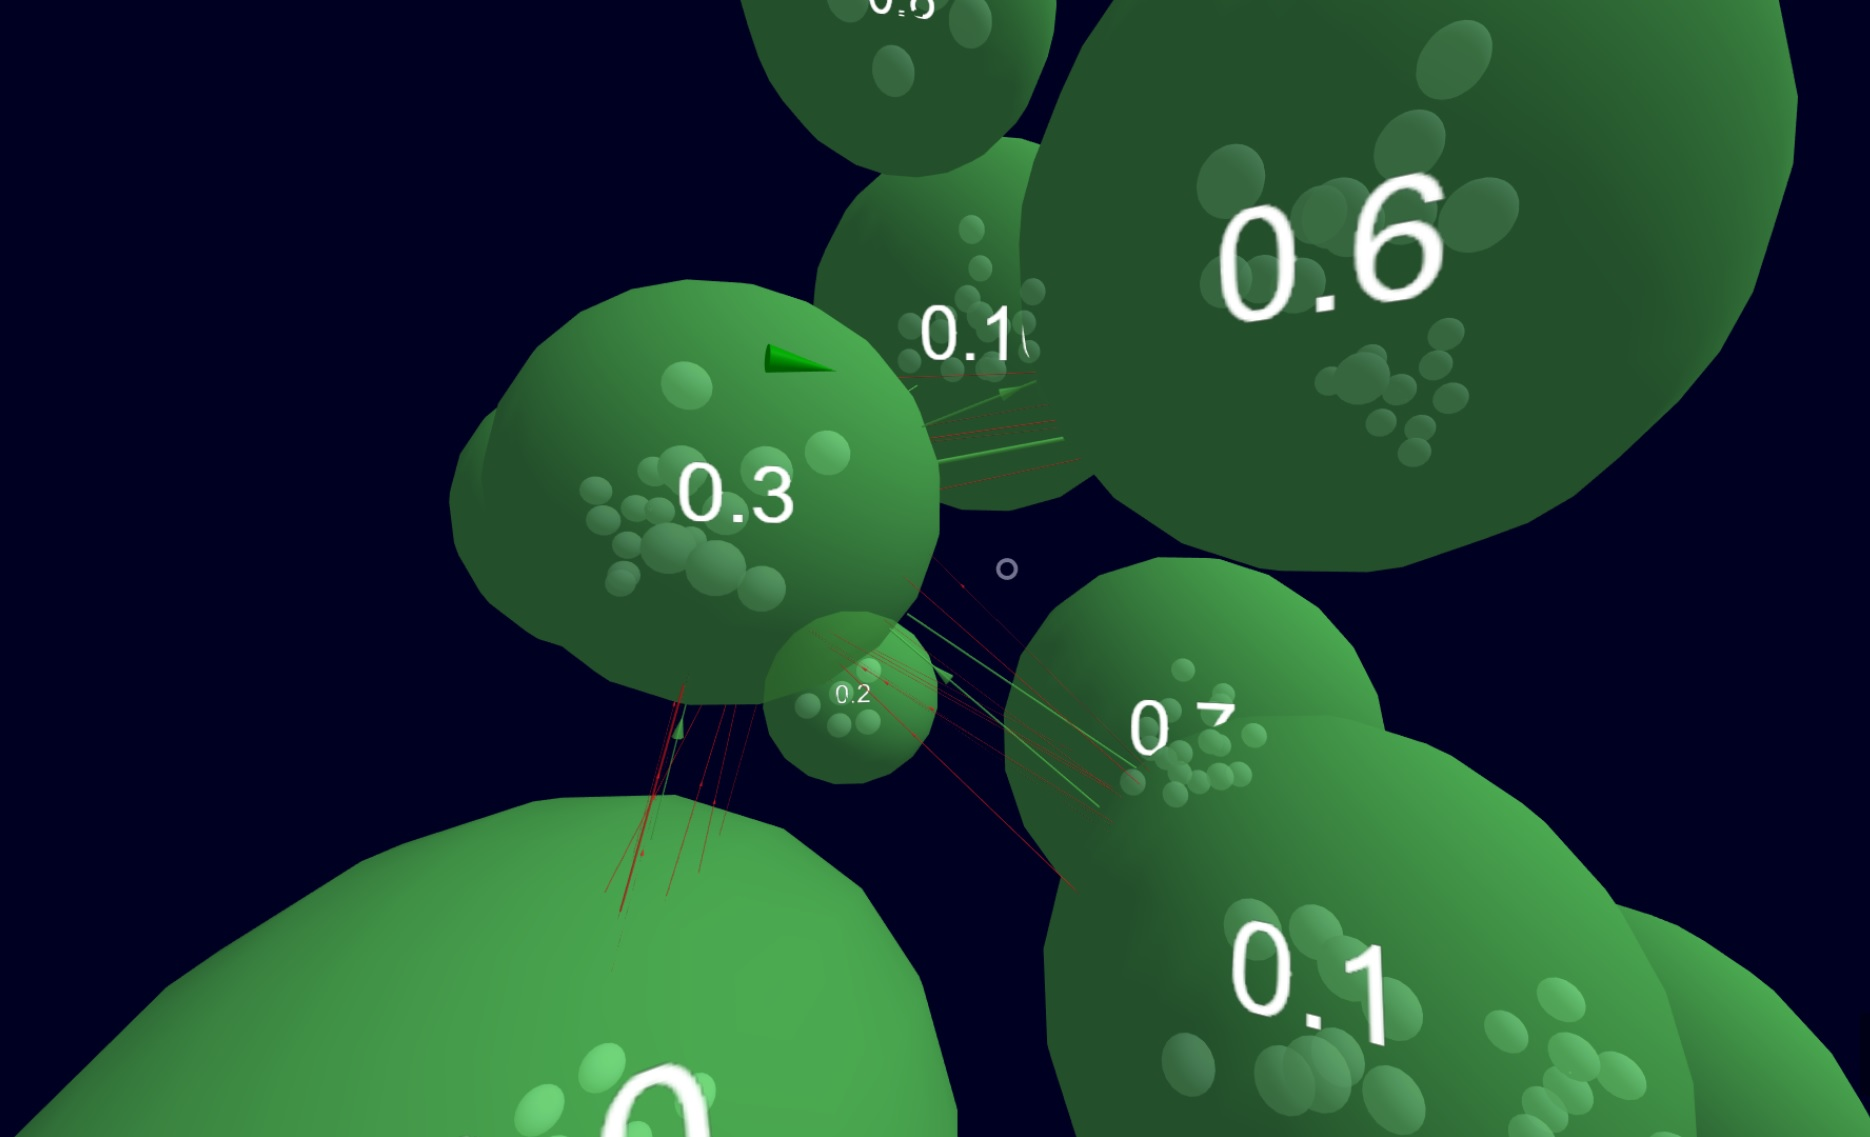
\includegraphics[width=1\textwidth]{graphics/conceptScreenshot.jpg}
    \caption[Screenshot of the comorbidity network dataset.]{Screenshot of the comorbidity network dataset from \ref{fig:original2DdiseaseNet} in our hierarchical network visualization. On the screenshot only edges from node 0.3 are displayed.} % Remove the [...] argument if the original caption should be used in the figure list.
    \label{fig:conceptSketch} 
\end{figure}